\chapter{Model systemu}

Aplikacja \emph{TeamSync} działa w środowisku o rozproszonym charakterze --- wszyscy użytkownicy w systemie są postrzegani jako odrębne i niezależne węzły (stacje robocze) w pewnej określonej lokalizacji w sieci. Każdy z użytkowników posiada unikalny identyfikator jednoznacznie wskazujący na niego. Model zakłada, że istnieje pomiędzy wszystkimi parami użytkowników łączność, która może być przerywana i wznawiana w dowolnych momentach.

Dodatkowo, w systemie znajduje się element centralny --- serwer NTP \cite{ntp} \cite{ntparticle}, który odpowiada na komunikaty użytkowników, odsyłając im znaczniki czasowe serwerowego czasu w momencie odebrania żądania. Serwer NTP zapewnia swoją dostępność za pomocą replikacji wewnątrz własnej ustrukturyzowanej sieci i w powyższym modelu zakładana jest jego bezawaryjność.

\begin{figure}[htb]
  \vspace{5pt}
  \begin{center}
    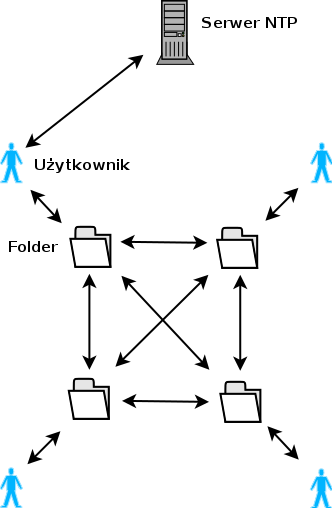
\includegraphics[width=200pt]{figures/model.png}
  \end{center}
  \caption{Model systemu \emph{TeamSync}.}
\end{figure}

Komunikacja i wymiana danych pomiędzy użytkownikami zachodzi tylko i wyłącznie poprzez aplikację BitTorrent Sync. Wymiana danych odbywa się automatycznie w momencie umieszczenia przez użytkownika nowych plików we wskazanym wcześniej folderze, lub w chwili modyfikacji już istniejących danych wewnątrz niego. Na poziomie transportu danych, jest on realizowany za pomocą protokołu BitTorrent.

Głównym obiektem, wewnątrz którego dane są obustronnie synchronizowane, jest folder --- w dalszej części pracy zastępowany również słowem ,,katalog'' o tożsamym znaczeniu. Po synchronizacji folderów każdy z węzłów posiada pełną kopię uwspólnianych danych wewnątrz swojego lokalnego folderu. Użytkownicy łączą wzajemnie swoje katalogi poprzez podanie ciągu 32 znaków (jest to tzw. \emph{secret}), za pomocą którego narzędzie BitTorrent Sync na jednym węźle jest w stanie odszukać u innego użytkownika zdalny folder, który oznaczony jest tym samym \emph{secretem}. 

System BitTorrent Sync gwarantuje natychmiastowe rozpoczęcie synchronizacji wszystkich danych wewnątrz folderu pomiędzy grupą połączonych ze sobą użytkowników. Wymiana danych pomiędzy dwoma węzłami odbywa się bezpośrednio --- bez serwera --- i nie jest możliwa, jeśli nie mają one możliwości nawiązania połączenia. Dodatkową konsekwencją takiej sytuacji jest fakt, że aby rozpropagowanie modyfikacji danych w sieci mogło mieć miejsce, przynajmniej dwaj użytkownicy muszą być do niej podłączeni.

Katalog synchronizowany przez użytkowników jest folderem zawierającym dowolną ilość danych, ograniczoną wyłącznie przez ilość dostępnej pamięci w systemie operacyjnym użytkownika. Pliki i katalogi wewnątrz współdzielonego folderu mogą być dowolnego typu, a dowolność ich nazw ogranicza jedynie system operacyjny.

\section*{Spójność wymienianych danych}

Użytkownicy synchronizujący ze sobą dane wewnątrz folderów --- ze względu na częstą zmianę dostępności każdego z węzłów --- narażeni są na wiele sytuacji grożących brakiem spójności wymienianych danych. Każdy z użytkowników posiada swoją lokalną, pełną kopię uwspólnionych plików. Podczas modyfikacji jednego z nich, zmiany rozsyłane są do pozostałych \emph{obecnych w danym momencie w sieci} węzłów --- w przypadku nieobecności dowolnego z użytkowników, zmiana zostanie odłożona w czasie do momentu, w którym będzie on dostępny w sieci. Wówczas --- o ile dowolny z węzłów posiadający dane po zmianie również jest obecny w sieci --- zmiany zostają natychmiast rozpropagowane.

Dodatkowo im więcej węzłów posiadających zmodyfikowane dane jest w sieci, tym szybciej dane będą się synchronizować. Dzieje się tak dlatego, że do transportu użyto protokołu \emph{BitTorrent}, za pomocą którego pobierane są drobne fragmenty danych od wszystkich dostępnych węzłów je posiadających, a dopiero po pobraniu fragmentów następuje łączenie ich w całość. Pozwala to na znacznie szybszą i bezpieczniejszą wymianę danych pomiędzy użytkownikami wewnątrz systemu \emph{BitTorrent Sync}, ponieważ fragmenty danych pobierane są od pozostałych węzłów równolegle.

Jednak pomimo cennych korzyści, podstawową trudnością jest zachowanie spójności w rozproszonym systemie. \emph{BitTorrent Sync} gwarantuje, że po uspójnieniu danych przez wszystkich użytkowników w systemie --- niezależnie od wcześniejszych różnic w przechowywanych lokalnie danych --- wszyscy użytkownicy ostatecznie będą posiadali \emph{jednakową} kopię danych. Ich lokalne zmiany, które nie zostały rozpropagowane w sieci zostaną dodane do katalogu \texttt{.sync} wewnątrz synchronizowanego katalogu, aby nie utracili oni swoich wersji zmodyfikowanych danych. Zawartość katalogu \texttt{.sync} nie jest przesyłana w sieci --- każdy węzeł ma inną jego zawartość.

\section*{Komunikacja między użytkownikami}

Podstawowymi obiektami, za pomocą których użytkownicy mogą się porozumiewać, są komentarze. Komentarz można umieścić w systemie \emph{TeamSync} za pomocą interfejsu graficznego, który dodaje go w odpowiedni sposób do systemu plików synchronizowanego folderu i rozsyła do pozostałych węzłów w sieci. Komentarz może zostać umieszczony w systemie przez dowolnego użytkownika, natomiast fizycznie w systemie przechowywany jest jako plik (na jeden komentarz w systemie przypada jeden plik) zawierający w sobie takie informacje jak:

\begin{itemize}[noitemsep]
 \item treść wypowiedzi,
 \item data i czas zamieszczenia,
 \item identyfikator autora,
 \item listę osób, które odczytały komentarz,
 \item historię zmian (poprzednia treść oraz data i czas zmiany).
\end{itemize}

Komentarze --- w dalszej części pracy nazywane również ,,wypowiedziami'', lub ,,postami'' --- zgrupowane są w większe struktury nazwane wątkami. Jeden wątek --- w dalszej części pracy nazywany też ,,dyskusją'' --- może zawierać w sobie nieograniczoną ilość wypowiedzi i może zostać oznaczony w systemie jako dyskusja na temat konkretnego (wybranego przez autora wątku) pliku znajdującego się w folderze.

W systemie wątek reprezentowany jest przez specjalnie oznaczony (za pomocą jego nazwy) katalog, wewnątrz którego znajdują się pliki z komentarzami. Dodatkowo, wewnątrz folderu przechowującego wątek, pomiędzy plikami z komentarzami znajduje się plik zawierający podstawowe informacje o wątku, między innymi:

\begin{itemize}[noitemsep]
 \item tytuł dyskusji,
 \item identyfikator autora,
 \item data i czas rozpoczęcia watku,
 \item plik, którego wątek dotyczy.
\end{itemize}

\begin{figure}[htb]
  \vspace{5pt}
  \begin{center}
    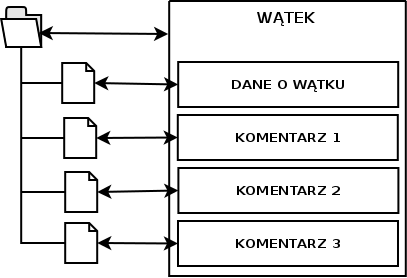
\includegraphics[width=240pt]{figures/folder-thread.png}
  \end{center}
  \caption{Odwzorowanie fizycznego składowania plików z komentarzami w wątku na logiczną ich reprezentację w systemie.}
\end{figure}

Na powyższym rysunku zaprezentowano, w jaki sposób fizycznie przechowywane są komentarze i w jaki sposób logicznie udostępniane są użytkownikom w systemie. Na jego podstawie można opisać kolejne założenie systemu, stanowiące o tym, że nie ma możliwości, aby w systemie komentarze istniały bez wątku --- przynależność wypowiedzi do dyskusji jest obligatoryjna.

Użytkownik może mieć wiele (maksymalnie $10$) folderów współdzielonych, każdy z innymi węzłami. Z tego powodu w modelu uwzględniono tzw. ,,tożsamości''. Tożsamość to nazwa użytkownika wpisywana przez niego podczas dołączania do folderu, która jest wyświetlana innym użytkownikom. Jedna tożsamość obowiązuje w jednym folderze i nie ma ograniczeń dotyczących powtarzalności --- użytkownik może w każdym uwspólnianym folderze mieć identyczną wyświetlaną nazwę.

Model systemu zakłada, że pliki raz zamieszczone w folderze nie będą zmieniać swojej lokalizacji wewnątrz niego. Założenie to może nie być przestrzegane tylko w przypadku, gdy żaden z wątków nie dotyczy przenoszonego pliku. W przeciwnym wypadku --- jeśli plik zmieni lokalizację (nawet pozostając nadal w uwspólnionym folderze) albo nazwę --- dyskusja dotycząca pliku nie zostanie wyświetlona. Powyższe założenie nie wnosi negatywnego działania w odniesieniu do synchronizowanych danych --- dotyczy wyłącznie funkcjonalności komentowania.

Wszystkie dane służące do obsługi systemu \emph{TeamSync} --- komentarze, pliki z danymi wątku, pliki przechowujące informacje o użytkownikach, pliki konfiguracyjne --- zapisywane są w formie słownika według formatu \texttt{JSON}. Każdy ze słowników zawiera klucze (ciągi znaków określające daną właściwość) oraz ich wartości.